\subsection{Effect of the Courant limit}

In function of the FDTD model, a discretization was performed of course, both in time and space. To justify the model physically, the steps in both time and space have to be chosen small enough. \\
The step in space $\Delta z$ has to be small enough to get rid of the wave phenomena. It cannot cross the boundary value of $\frac{\lambda_{min}}{10}$. The minimal wavelength $\lambda_{min}$ is simple to calculate as the fraction of the wave speed and the maximal frequency. The maximal frequency is given by the bandwith of the signal: $\frac{1}{\pi \tau_r}$. Considering the default settings ($\tau_r = 40.0e-12 s$ and $v = 200.0e6 m/s$) is the maximal step in space equal to $2.5133$ mm. Results with a bigger step in space can be ignored as they are physically incorrect.



The Courant limit is introduced to determine the maximal step in time. This limit states that $\Delta t$ can not be bigger than $\frac{\Delta z}{v}$. Just as in the case of $\Delta z$, results for $\Delta t$ bigger than this limit can be neglected since the time step $\Delta t$ will be bigger than the time it takes for the wave to cover a distance $\Delta z$ in that case. To illustrate this, the time step was brought up to $11e-12 s$ and the none converging graph is shown in figure~\ref{fig:test}.

\begin{figure}[! h]
\centering
\begin{subfigure}{.5\textwidth}
  \centering
  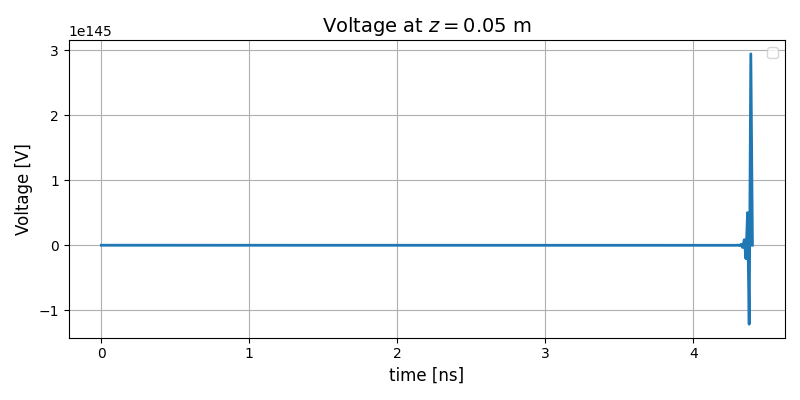
\includegraphics[width=.9\linewidth]{figures/alpha=1.1(z).png}
  \caption{Voltage for $\alpha = 1.1$ at $z = 0.05m$}
  \label{fig:dt1}
\end{subfigure}%
\begin{subfigure}{.5\textwidth}
  \centering
  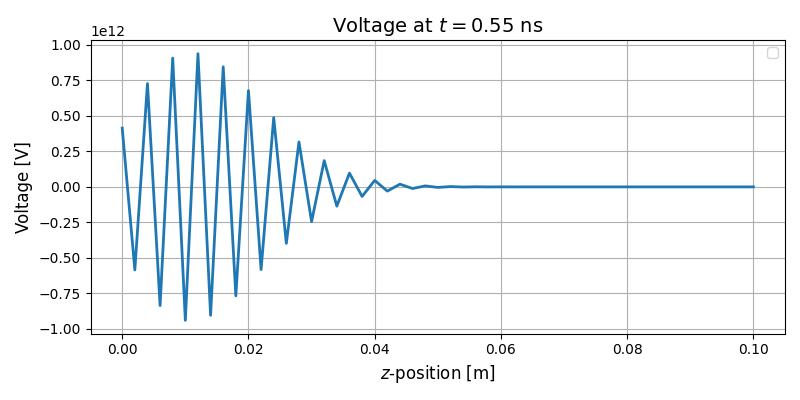
\includegraphics[width=.9\linewidth]{figures/alpha=1.1(t).png}
  \caption{Voltage for $\alpha = 1.1$ at $t = 0.55ns$}
  \label{fig:dt2}
\end{subfigure}
\caption{}
\label{fig:test}
\end{figure}

Applying the default values, $\Delta t$ exactly satisfies the Courant limit. This is the so called magic time step $(v\Delta z = \Delta t)$. When a time step smaller than the magic one is chosen, Gibbs phenomena occur.



The Courant factor $\alpha$, which also appears in the update equations, shows in what extend Gibbs phenomena are present. The maximal value of the Courant factor (to be physically relevant) is 1, which is also the perfect case. The lower the Courant factor becomes, the more Gibbs phenomena occur. This is illustrated in Figure~\ref{fig:alpha} for $\alpha$ being respectively 0.99 and 0.90. 

\begin{figure}[! h]
\centering
\begin{subfigure}{.5\textwidth}
  \centering
  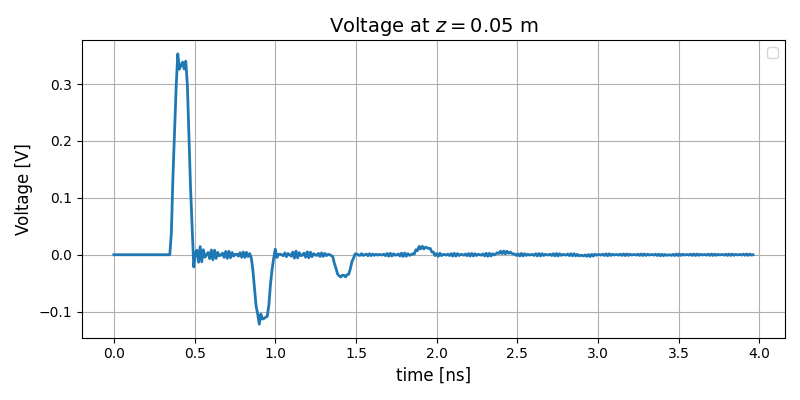
\includegraphics[width=.9\linewidth]{figures/alpha=0.99.png}
  \caption{$\alpha = 0.99$}
  \label{fig:dt1}
\end{subfigure}%
\begin{subfigure}{.5\textwidth}
  \centering
  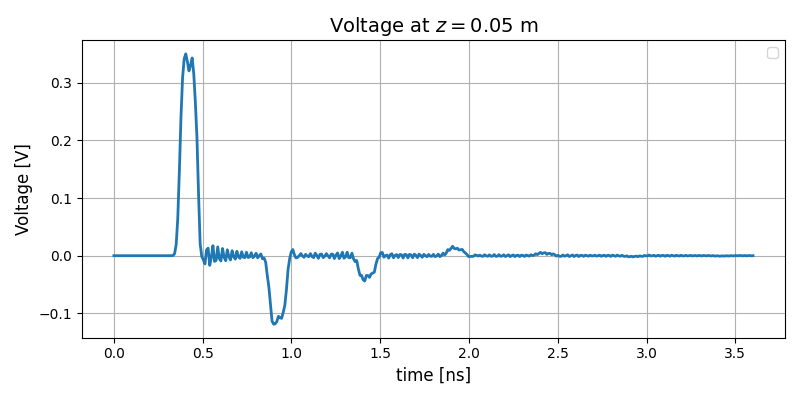
\includegraphics[width=.9\linewidth]{figures/alpha=0.90.png}
  \caption {$\alpha = 0.90$}
  \label{fig:dt2}
\end{subfigure}
\caption{}
\label{fig:alpha}
\end{figure}